\section{ARCADIA-MD1}

ARCADIA-MD1 is an LFoundry chip which implements the technology 110 nm CMOSS node
with six metal layer \ref{articolo fully depl}.
The standard p-type substrate was replaced with an n-type floating zone material,
that is a tecnique to produce purified silicon crystal. (pag 299 K.W.).\\

Wafer thinning and backside litography were necessary to introduce a junction
at the bottom surface, used to bias the substrate to full depletion while
maintaining a low voltage at the front side.  \\
C'è un deep pwell per - priority chainseparare l'elettronica dal sensore; per controllare il punchthought
è stato aggiunto un n doped epitaxial layer having a resistivity lower than the substrate.

RILEGGI SUL KOLANOSKY COS'È IL PUNCHTHROUGHT, FLOAT ZONE MATERIAL, COME VENGONO FATTI I MAPS
COME FAI LE GIUNZIONI

\begin{figure}
\centering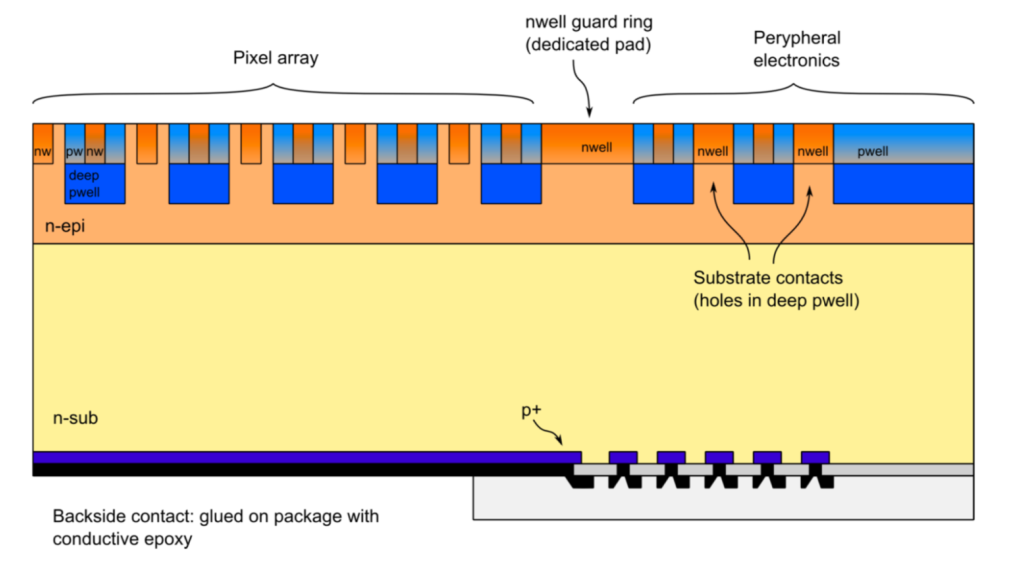
\includegraphics[width=8cm]{figures/pixel_scheme.png}
\caption{Concept cross section of one pixel}
\label{fig:pixel_scheme}
\end{figure}

It is part of the cathegory of DMAPS
Small electrode to enhance the signal to noise ratio.

It is operated in full depletion with fast charge collection by drift.

Prima SEED si occupa di studiare le prestazioni: oncept study with small-scale test structure (SEED),
dopo arcadia: technology demonstration with large area sensors
Small scale demo SEED(sensor with embedded electronic developement)
Quanto spazio dato all'elettronica sopra il pwell e quanto al diodo. ..



\subsection{Matrix division}
The matrix is divided into an internal physical and logical hierarchy:
The 512 columns are divided in 16 section: each section has different voltage-bias + serializzatori.
Each section is devided in cores () in modo che in ogni doppia colonna ci siano 1Pacchetto dei dati
6 cores. ricordati dei serializzaatori: sono 16 ma possono essere ridotti ad uno in modalità spazio

Questa divisione si rispecchia in come sono fatti i dati: scrivi da quanti bit un
dato è fatto e le varie cordinate che ci si trovano dentro; devi dire che c'è un pixel hot
e spieghi dopo a cosa serve, e devi accennare al timestamp

"A core is simply the smallest stepped and repeated instance of digital circuitry.
A relatively large core allows one to take full advantage of digital sybthesis tools
to implement complex functionality in the pixel matrix, sharing resources among
many pixels as needed.".
pagina 28 della review.\\




TABELLA: con la gerarchia del chip
Matrix (512x512 pixels)
Section (512x32 pixels)
Column (512x2)
Core (32x2)
Region (4x2)

Nel chip trovi diverse padframe: cosa c'è nelle padframe e End of section.

"DC-balance avoids low frequencies by guaranteeing at least one transition every
n bits; for example 8b10b encoding n =5"


\subsection{Front end description}
ALPIDE (ALice PIxel Detector) like.
Spiegazione del circuito. Articolo di Kim perfetto + tesi di Moustakas.
Come possiamo cambiare i parametri del FE.
